\documentclass[11pt, a4paper]{article}
\usepackage[greek,english]{babel}
\usepackage[linesnumbered,ruled]{algorithm2e}
\usepackage{amsmath, amssymb, fullpage}
\usepackage{graphicx}
\usepackage[titletoc,title]{appendix}
\usepackage[section]{placeins}
\usepackage{enumerate}
\usepackage{float}
\graphicspath{{./img/}}
\setcounter{tocdepth}{4}
\linespread{1}
\title{
	\begin{figure}[H]
  		\centering
      	
\includegraphics[width=0.4\textwidth]{SFU_logo.jpg}
	\end{figure}
	~\\
	\large CMPT711 Bioinformatics Algorithms~\\Course Project D ~\\~\\~\\
	\Huge\textbf{Understanding Metabolic Network Models~\\~\\}}
\author{Hooman Zabeti\\301348564\and Yiji Wang\\301286922\and Peiyu Cui\\301345033\and Haihong Tang\\301268397}
\date{~\\Supervised by~\\Prof. Leonid Chindelevitch~\\~\\December 15th, 2017}
\begin{document}
	\nocite{*}
    \maketitle
    \thispagestyle{empty}
    ~\\
    %==========Abstract==========%
    \begin{abstract}
    ~\\In this project, we learned about the constraint-based models as the only methodology that allows the study of metabolism at the whole-genome scale and flux balance analysis which is commonly used analyse constraint-based models. There are two popular toolboxes that are based on flux balance analysis, Cobra from UCSD published in 2007 and Mongoose from MIT in 2014. Cobra uses floating arithmetic for computation while Mongoose introduces a breakthrough method using exact arithmetic. Theoretically Mongoose should give better results with its basis on exact arithmetic, especially for those models with small integer fractions. In order to find out which tool performs better exactly, we performed experiments on these two tools using 80 BIGG models including 2 yeast models from UCSD repository and compared them using the results in terms of accuracy and analysis time.
    \end{abstract}
    \newpage
    \linespread{2}
    \tableofcontents
    \thispagestyle{empty}
	\newpage
	\linespread{1}
	%==========Introduction==========%
	\section{Introduction}
	\setcounter{page}{1}
	~\\A metabolic network (MN) is the sum of all biochemical processes that determine the physiological and biochemical properties of a cell$\cite{Chalancon1}$. In particular, these processes often encompass two or more molecules' (reactants) interactions. As such, these networks consist of the chemical reactions of metabolism, the metabolic pathways, and the regulatory interactions. Recent progress in genome annotations and the advancement of genomics have made the extraction of metabolism-related information possible at a genomics scale$\cite{Feist2}$. This results in great efforts on network reconstruction and predictive model building. Furthermore, there are several strategies to model the metabolic network; for example, kinetic model, constraint-based model, topological analysis, and flux balance analysis.

	~\\Kinetic modelling is a mathematical modelling technique attempting to compensate for the lack of explicit kinetics by exploring the entire parameter space at a predefined steady state of the metabolites. Constraint-based model is another mathematical approach in which the outcome of each decision is constrained by a minimum and maximum range of limits, thereby allowing fast calculations of large networks under the steady state assumption$\cite{Conde3}$. Topological analysis could reveal the evolution history and design principle of the metabolic network to some extent. Flux balance analysis is a mathematical approach for analyzing the flow of metabolites through a metabolic network, thereby making it possible to predict the growth rate of an organism or the rate of production of a bio-technologically important metabolite$\cite{Orth12}$.

	~\\This article aims to provide a detailed comparison of two toolboxes, Cobra and Mongoose, when computing these models and analysis, and the techniques being explored to efficiently accelerate their computation.

	~\\This paper is organized as follows:
	\begin{itemize}
	    \item Section 2 provides related works and methods on the context of Cobra and Mongoose toolboxes.
	    \item Section 3 gives definitions and explanations of Flux Balance Analysis (FBA) and blocked reactions.
	    \item Section 4 describes a detailed analysis and computational results of Cobra and Mongoose toolboxes, and the various optimization used to improve throughput and energy without impacting application accuracy.
	    \item Section 5 describes the key metric that should be considered when modelling the metabolic network.
	\end{itemize}
	\newpage
	%==========Related Work==========%
	\section{Related Work}
	\subsection{Cobra}
	~\\In this subsection, we describe the position of Cobra toolbox in the context of metabolic network analysis and some of the concepts that motivated its development. We will also present a brief chronology of the major steps in its history, and some current domains to which it is being applied.

	~\\The Cobra toolbox, a Matlab package for implementing constraint-based reconstruction and analysis (COBRA) methods, lowers the barrier of entry for biologists to use the powerful COBRA methods. Its first release is in 2007 along with a variety of useful analysis methods, including flux balance analysis, gene essentiality analysis, and minimization of metabolic adjustment analysis. Since the release of the first version of the Cobra toolbox, many additional Cobra-related methods have been published [4 - 6], and in 2011, version 2 of Cobra toolbox was released with an extended capability to perform geometric flux-balance analysis$\cite{Smallbone7}$, loop law$\cite{Schellenberger8}$, and Monte Carlo sampling$\cite{Thiele9}$ \textit{etc.}. The Cobra toolbox can also easily be interfaced with other software tools for analyzing metabolic networks and fluxes in Matlab that complement the Cobra toolbox$\cite{Klamt10}$. Although the Cobra toolbox can handle any reasonable input format with some modification for the models, we will describe the model input using the Systems Biology Markup Language (SBML) format$\cite{Hucka11}$; we distribute all of our models in this format.

	~\\Many applications can benefit from applying Cobra toolbox. In the following, we will provide examples of areas where Cobra toolbox are currently making an impact and highlight emerging areas where Cobra toolbox will make an impact in the future.

	~\\Thorleifsson \textit{et.al} present a Cobra toolbox extension, rBioNet, enabling the construction of publication-level biochemical networks while implementing important quality control and assurance measures, which are crucial for the construction of high-quality genome-scale biochemical networks$\cite{Thorleifsson13}$. In particular, it puts emphasis on a user-friendly interface that allows novices to Matlab performing high-quality metabolic reconstructions. It consists of three parts: a metabolite creator with associated metabolite database; a reconstruction creator; and a reaction creator with reaction database.

	~\\Fleming \textit{et.al} introduces an extension, named von Bertalanffy, of the Cobra toolbox for quantitative assignment of stoichiometric model reaction directionality via integration of experimentally derived$\cite{TZimmerman14}$ and group contribution estimates of standard Gibbs energies of formation$\cite{Jankowski15}$ and reactant concentrations. It automatically generates extensive statistics and figures, focusing on quantitative reaction directions that disagree with reconstruction directions. Since Cobra toolbox supports model exchange via the SBML, this extension may be applied to an arbitrary mass and charge-balanced metabolic reconstruction.

	~\\Kostromins \textit{et.al} proposes the Paint4Net, a novel Cobra toolbox extension for automatic generation of a hypergraph layout of defined scope with the steady state rates of reaction fluxes of stoichiometric models$\cite{Kostromins16}$. Fluxes of reactions and directionalities are constantly represented in the visualization while detailed information about reaction (\textit{e.g.} ID, name, synonyms, and formula) and metabolite appears placing the cursor on the item of interest. In addition, Paint4Net functionality could be utilized to: (1) obtain list of involved metabolites and dead-end metabolites of the visualized part of the network, (2) filter certain metabolites from representation (3) inspect isolated parts of a metabolic network (4) investigate running cycles when all the substrates are cut down.

	~\\Mao \textit{et.al} presents a Cobra toolbox extension named ORCA, which extends the scope of established constraint-based reconstruction and analysis metabolic modelling and includes three unique functionalities: a dynamic flux balance analysis framework along with kinetic constraints; metabolic pathway identification with futile loop elimination; and a framework integrating three analyses on multi-objective optimization, robustness analysis, and fractional benefit analysis$\cite{Mao17}$. It conducts flux balance analysis based methods to multi-objective formulation and extends the robustness analysis of Cobra into a framework context. It also has a simple algorithm to exclude the futile fluxes generated during flux balance analysis and allows identification of the pathways belonging to the metabolite of interest.
	\subsection{Mongoose}
	~\\In this subsection we will discuss the position of Mongoose toolbox in the context of metabolic network analysis and some of the ideas that drove its development. We will also explore some current domains to which it is being applied.

	~\\The Mongoose (MetabOlic Network GrOwth Optimization Solved Exactly)toolbox developed by Chindelevitch \textit{et.al}$\cite{Leonid19}$, a Matlab package for analyzing the structure of constraint-based metabolic models in exact arithmetic, solves the inconsistency problem that is caused by floating-point arithmetic. In other words, the results of flux balance analysis vary with the applications being used; however, Mongoose toolbox could produce consistent results by utilizing exact arithmetic. This is because its core is an exact arithmetic-based algorithmic pipeline that has a structural analysis supported by new theoretical results. Furthermore, the structural analysis performed by Mongoose will converge after a single cycle which allows the user to perform further analyses, such as the identification of minimal media, essential genes, and synthetic lethal reactions on a model \textit{etc.}. Therefore, when compared to Cobra, Mongoose shows a significant improvements. It especially could produce certifiably consistent and reproducible results, while leveraging its structural insights to convert many intractable problem in metabolic network analysis.

	~\\Although the exact arithmetic technique employed by Mongoose will require more computation resources, the computation resources never exceeds an order of magnitude. The small increase of consumption on computation resource could be compensated by the significant reduction of the size of the metabolic network which will later speed up all subsequent analyses.

	~\\Many applications could obtain benefits from using Mongoose toolbox. In the following, we will examine some examples of areas where Mongoose toolbox are currently making an impact. Chindelevitch \textit{et.al} utilized Mongoose toolbox to perform analysis on identification of blocked reactions and prediction of essential genes when his team researched on MetaMerge, an algorithm for semi-automatically reconciling a pair of existing metabolic network reconstructions into a single metabolic network model$\cite{Leonid21}$. Chindelevitch \textit{et.al} proposes that Mongoose toolbox could be offered as a model verification platform, which will be useful in identifying errors in model functionality and helping curators to debug them$\cite{Leonid22}$. Its exact arithmetic can also make an improvements on the results of the analysis of genome-scale metabolic network models$\cite{Leonid21}$.
	\newpage
	%==========Methods==========%
	\section{Methods}
	
	~\\ In this section we explain important conditions and methods we need for the next section.\\
	
	~\\\textbf{Constraint-base} models have two assumptions$\cite{Leonid20}$. First assumption is the system should be in the \textbf{quasi-steady-state} (or steady-state for short). That means, we are analyzing the system in a time period when we can assume we are not having any changes in metabolite concentrations (i.e., production and consumption rates of metabolites are equal to each other). The advantage of this assumption is we do not need information on metabolite concentrations of their change rates. Therefore if $S$ be the model's stoichiometric matrix and $v$ be a vector of fluxes, this assumption implies 
	$$Sv=0$$
	~\\The second assumption is an irreversible reaction can only have a non-negative flux assuming that the system is in its steady-state. Hence, if $\mathcal{I}$ be the set of irreversible reaction we have 
	$$v_i\geq 0\text{ , } \forall i \in \mathcal{I}$$

	~\\Notice that the constraints in constraint-based model will provide the feasible solution space for us, In order to find the optimal solution we need \textbf{Flux Balance Analysis}. FBA can be used to predict the growth rate of cell under different conditions$\cite{Leonid19}$. FBA is using linear programming to obtain the solution for desirable result and in general is in the following form$\cite{Orth12}$
	\begin{align*}
	&\max(\min)\hspace{.1in} c.v\\
	& \text{subject to:}\\
	&\hspace{.3in}Sv= 0\\
	& \hspace{.3in}\alpha_i\leq v_i \leq \beta_i
	\end{align*}
	where $c$ is the vector of weights which depend on our problem. For instance in order to find the growth rate $c$ would be all zeros except on indexes correspond to biomass reactions ($c_{biomass}=1$). Also, $\alpha_i$'s and $\beta_i$'s are lower and upper bound of vector of fluxes. For instance based on second assumption of constraint-based models $\alpha_i\geq 0$ for every $i\in \mathcal{I}$.

	~\\In a metabolic network, reactions which cannot obtain a non-zero flux due to the steady-state assumption and the non-negative constraints for irreversible reactions contained in the network, are called \textbf{blocked reactions}$\cite{Leonid19}\cite{Leonid20}$. i.e., if $S$ be the networks stoichiometric matrix and $\mathcal{I}$ be set of irreversible reactions then for reaction $i$ satisfaction of following constraints
	$$Sv=0 \text{ and }v_i\geq 0 \text{ , } \forall i\in \mathcal{I}$$
	Implies $v_i=0$.\\

	~\\Both COBRA and MONGOOSE are able to identify blocked reaction. However, MONGOOSE, in addition to identifying blocked reactions, is able to categorize the blockage into three groups based on the blockage reason. Moreover, MONGOOSE is able to identify semi-blocked reactions and the effective and defective direction of such reaction$\cite{Leonid19}$.

	~\\The first type of blockage is \textbf{topologically blocked} reactions. The topological blockage may be caused by a reaction $i$ which contains a unique metabolite in the network. In this case, the mass balance condition (steady-state assumption) would imply $v_i=0$ $\cite{Leonid20}$.

	~\\This means the flux corresponds to such reaction is 0. Since this type of blockage is caused by the topology of the network, MONGOOSE categories these reactions as topologically blocked reactions$\cite{Leonid19}$.

	~\\The second type of blockages is \textbf{stoichiometrically blocked} reactions. This blockage would happen when without having non-negativity constraints we have $v_i=0$ for some $i$'s$\cite{Leonid20}$.

	~\\That means, with assumption that $S$ not a full row rank matrix, we do not have a non-trivial right null vector such that the flux corresponds to reaction $i$ is not 0. We can interpret this behavior as there exists at least a metabolite which the stoichiometry of that metabolite in a reaction is linearly independent of the stoichiometry of that metabolite in other reactions. Therefore if we have a non-zero flux corresponding to such reaction, we will end up with a \textbf{free lunches}. Note that set of the topologically blocked reactions is a subset of stoichiometrically blocked reactions. 

	~\\The third type of blockages is \textbf{irreversibility blocked} reactions. An irreversible blockage is caused if non-negative constraints for an irreversible reaction satisfied only if the flux corresponds to that reaction be 0$\cite{Leonid20}$.

	~\\Furthermore, MONGOOSE can identify a subset of reversible reactions which only satisfy our constraints in one direction. These reactions can be assumed as irreversible reactions since only one direction of them will be useful for us. In MONGOOSE, these reactions are known as pseudo-irreversible reactions, and they will be labeled as effectively forward or effectively backward based on their flux sign. In general, these reactions are called semi-blocked reactions$\cite{Leonid20}$.\\
	% ~\\\textbf{Constraint-base} models have two assumptions. First assumption is the system should be in the \textbf{quasi-steady-state} (or steady-state for short). That means, we are analyzing the system in a time period when we can assume we are not having any changes in metabolite concentrations (i.e., production and consumption rates of metabolites are equal to each other). The advantage of this assumption is we do not need information on metabolite concentrations of their change rates. Therefore if $S$ be the model's stoichiometric matrix and $v$ be a vector of fluxes, this assumption implies 
	% $$Sv=0$$
	% ~\\The second assumption is an irreversible reaction can only have a non-negative flux assuming that the system is in its steady-state. Hence, if $\mathcal{I}$ be the set of irreversible reaction we have 
	% $$v_i\geq 0\text{ , } \forall i \in \mathcal{I}$$

	% ~\\Notice that the constraints in constraint-based model will provide the feasible solution space for us, In order to find the optimal solution we need, \textbf{Flux Balance Analysis} can be used to analyzing the constraint-based model. For instance FBA can "be used to calculate the flow of metabolites through a metabolic network"$\cite{Hinton18}$. FBA can be used to predict the growth rate of cell under different conditions$\cite{Leonid19}$. 

	% \begin{align*}
	% &\max(\min)\hspace{.1in} c.v\\
	% & \text{subject to:}\\
	% &\hspace{.3in}Sv= 0\\
	% & \hspace{.3in}\alpha_i\leq v_i \leq \beta_i
	% \end{align*}

	% ~\\In a metabolic network, reactions which cannot obtain a non-zero flux due to the steady-state assumption and the non-negative constraints for irreversible reactions contained in the network, are called \textbf{blocked reactions}. i.e., if $S$ be the networks stoichiometric matrix and $\mathcal{I}$ be set of irreversible reactions then for reaction $i$ satisfaction of following constraints
	% $$Sv=0 \text{ and }v_i\geq 0 \text{ , } \forall i\in \mathcal{I}$$
	% Implies $v_i=0$.\\

	% ~\\Both COBRA and MONGOOSE are able to identify blocked reaction. However, MONGOOSE, in addition to identifying blocked reactions, is able to categorize the blockage into three groups based on the blockage reason. Moreover, MONGOOSE is able to identify semi-blocked reactions and the effective and defective direction of such reaction.

	% ~\\The first type of blockage is \textbf{topologically blocked} reactions. The topological blockage may be caused by a reaction $i$ which contains a unique metabolite in the network. In this case, the mass balance condition (steady-state assumption) would imply $v_i=0$.

	% ~\\This means the flux corresponds to such reaction is 0. Since this type of blockage is caused by the topology of the network, MONGOOSE categories these reactions as topologically blocked reactions$\cite{Leonid20}$.

	% ~\\The second type of blockages is \textbf{stoichiometrically blocked} reactions. This blockage would happen when without having non-negativity constraints we have $v_i=0$ for some $i$'s$\cite{Leonid20}$.

	% ~\\That means, with assumption that $S$ not a full row rank matrix, we do not have a non-trivial right null vector such that the flux corresponds to reaction $i$ is not 0. We can interpret this behavior as there exists at least a metabolite which the stoichiometry of that metabolite in a reaction is linearly independent of the stoichiometry of that metabolite in other reactions. Therefore if we have a non-zero flux corresponding to such reaction, we will end up with a \textbf{free lunches}. Note that set of the topologically blocked reactions is a subset of stoichiometrically blocked reactions. 

	% ~\\The third type of blockages is \textbf{irreversibility blocked} reactions. An irreversible blockage is caused if non-negative constraints for an irreversible reaction satisfied only if the flux corresponds to that reaction be 0$\cite{Leonid20}$.

	% ~\\Furthermore, MONGOOSE can identify a subset of reversible reactions which only satisfy our constraints in one direction. These reactions can be assumed as irreversible reactions since only one direction of them will be useful for us. In MONGOOSE, these reactions are known as pseudo-irreversible reactions, and they will be labeled as effectively forward or effectively backward based on their flux sign. In general, these reactions are called semi-blocked reactions.
	\newpage
	%==========Experiments and Results==========%
	\section{Experiments and Results}
%	\subsection{Cobra}
%	In order to learn how constraint-based models of bacterial metabolism are implemented using state of the art modeling tools, we utilizing the Cobra toolbox that was developed by Prof. Bernhard Palsson’s group at the University of California, San Diego in the Nature paper 'Quantitative prediction of cellular metabolism with constraint‐based models: the COBRA Toolbox.'$\cite{Becker20}$
%
%	~\\The goal of the first part of the laboratory is to load the SBML model of E. coli iJR904 and to evaluate its contents using\\$>>model=readCbModel('iJR904')$;\\After loading the model, we can identify (i) the number of genes(904), metabolites(761) and reactions(1075). (ii) the rank(743) of the resulting matrix\\$>>rank(full(model.S))$;\\(iii) degree of freedom(332) (i.e the extent to which the model is underdetermined)[x]\\$degree of freedom = number of reactions - rank of matrix$\\(iv) plot the matrix\\$>>spy(model.S)$.
%	\begin{figure}[H]
%  		\centering
%      	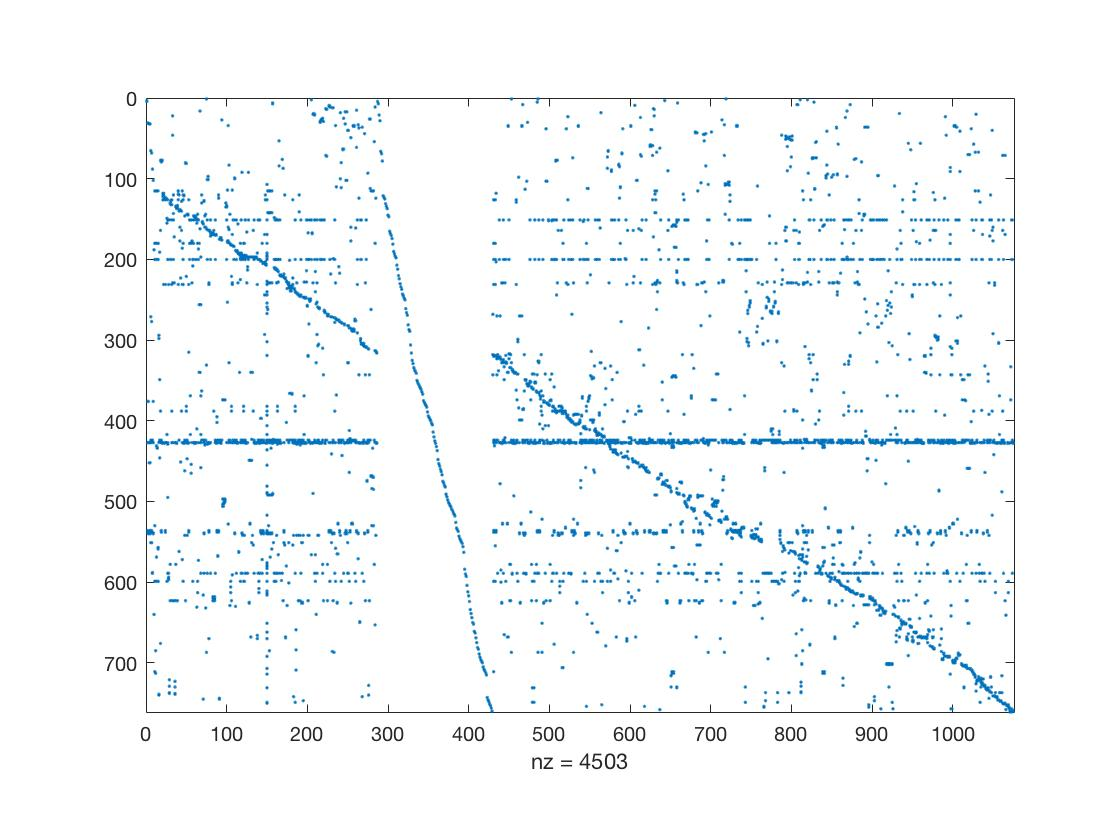
\includegraphics[width=1.0\textwidth]{matrix_plot.jpg}
%      	\caption{\textit{Plot of stoichiometry matrix where we can find highly connected metabolites.}}
%	\end{figure}
%	~\\Then we tried to solve the E. coli model using the FBA approach where the biomass maximization is the objective function.\\$>>solution1 = optimizeCbModel(model)$;\\
%	The growth rate is $0.9219 hr^{-1}$\\\\
%	Here we compare the biomass yield for different amount of glucose uptake.\\
%	$>>model2=changeRxnBounds(model,'EX\_glc\_\_D\_e',[-1],'l');$\\
%	Biomass yield is 0.0604389 when glucose uptake is $1 mmol/gdw hr$
%	and it increases linearly 0.539113 when glucose uptake is raised to $6 mmol/gdw hr$.\\
%	~\\Next we changed objective function for the linear programming problem to that of maximizing the rate of ethanol production to maximize ethanol yield\\
%	$>>model3=changeObjective(model,{'BiomassEcoli','EX\_etoh(e)'},[0,1]);$\\
%	we find the reaction is be under eraobic condition in this case and the growth rate is be 0.\\
%	~\\If we force the environment to be in anaerobic condition (i.e. set the oxygen taken to be 0)\\$>>model4=changeRxnBounds(model,'EX\_o2\_e',[0],'l');$\\We find that the ethanol yield is actually smaller than the result above, which means the maximum of ethanol yield may not be necessarily under anaerobic condition.\\
%	\begin{figure}[H]
%  		\centering
%      	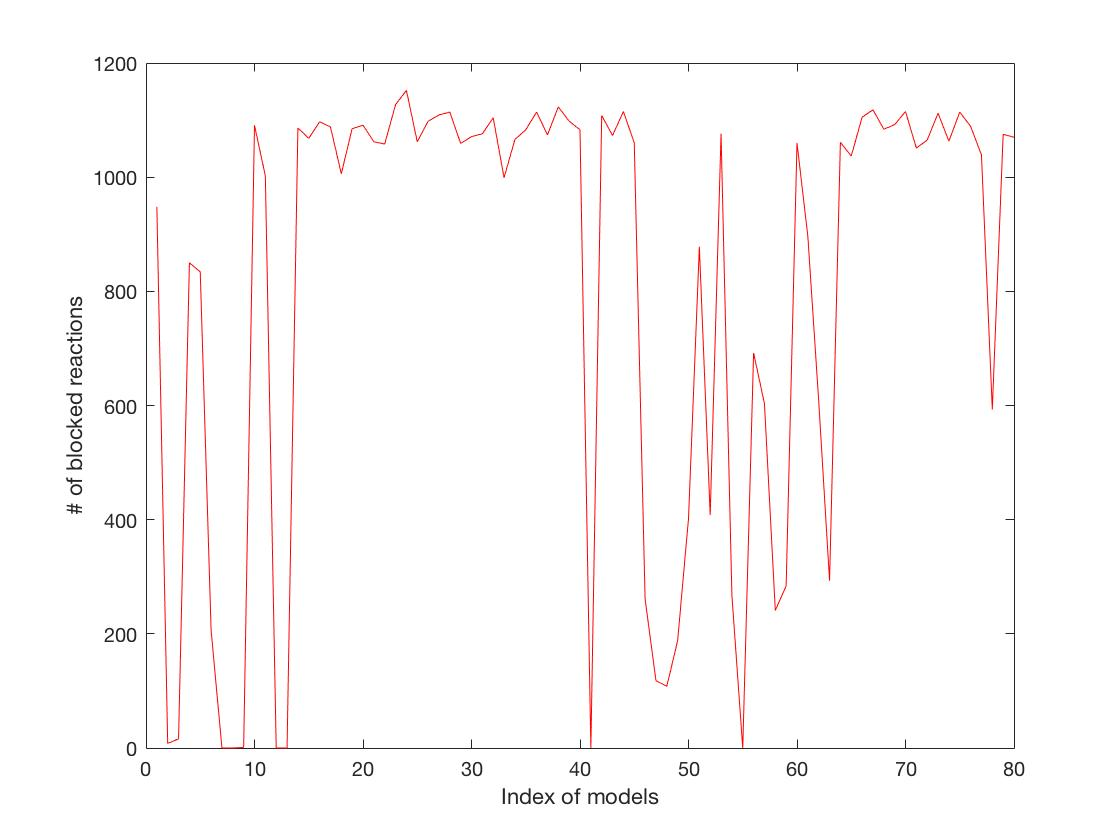
\includegraphics[width=0.8\textwidth]{cobra_all_model_reaction.jpg}
%      	\caption{\textit{Number of reactions for all models found by cobra.}}
%	\end{figure}
%	\begin{figure}[H]
%  		\centering
%      	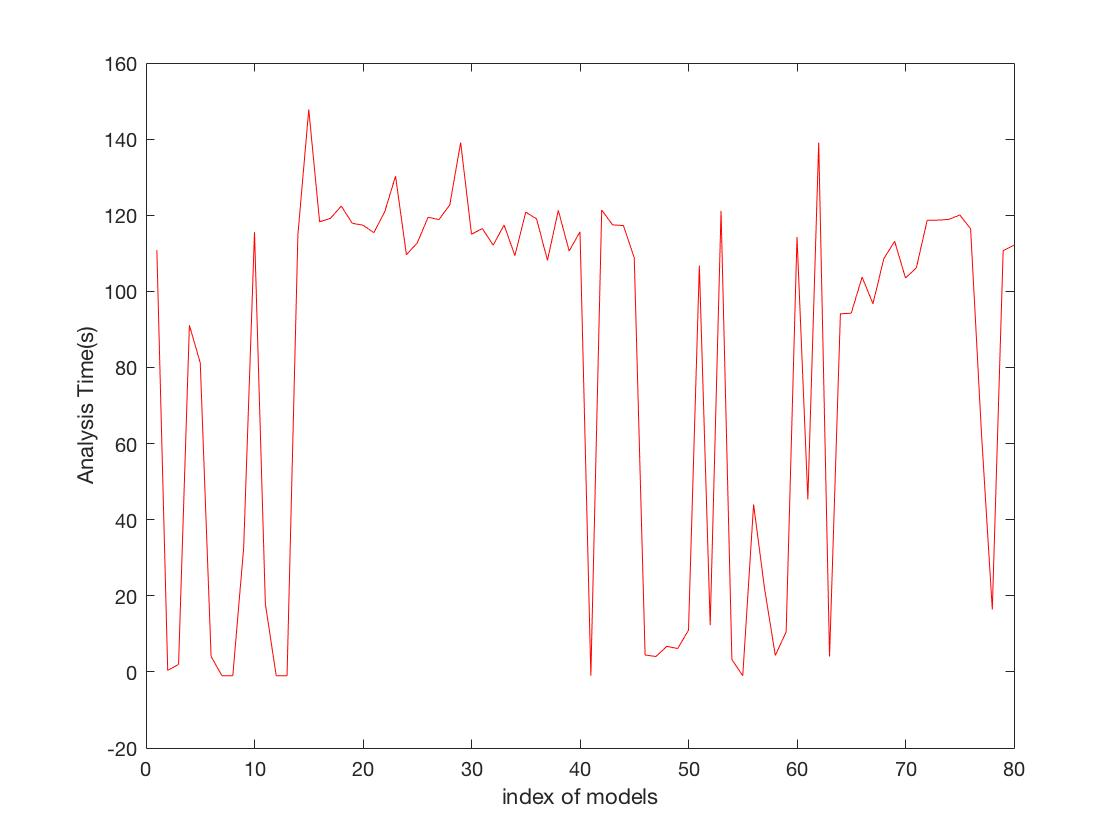
\includegraphics[width=0.8\textwidth]{cobra_all_model_time.jpg}
%      	\caption{\textit{Analysis time for all models by cobra.}}
%	\end{figure}
%	~\\After having a basic understading of FBA and cobra functions, we focused on the number of blocked reactions using yeast models iMM904, IND750 as gold standard data and all models from http://bigg.ucsd.edu/models. One interesting thing we find is that for some models, cobra cannot give the correct result in a reasonable time (e.g. 2 hours).
%	\begin{center}
%	\begin{tabular}{|c|c|c|} 
%	 \hline
%	 Yeast Model & \# Blocked Reactions & Analysis Time(s)\\
%	 \hline 
%	 iMM904 & 692 & 43.9767 \\
%	 IND750 & 603 & 22.0524 \\
%	 \hline
%	\end{tabular}
%	\end{center}
%	\subsection{Mongoose}
%	~\\In this section first we parsed and analyzed the structure of the model \textit{iJR904} of \textit{E. coli} with MONGOOSE. Then we repeat the same process for \textit{yeast} models \textit{iMM904} and \textit{IND750} as our gold standard models in order to compare results of COBRA and MONGOOSE. Finally, we repeat the same process for all 84 models available from the In Sili-co Organisms repository.
%
%	~\\For model \textit{iJR904} of \textit{E. coli} after parsing the model and reducing the network we obtained following results. This model contains 761 metabolites and 1075 reactions. Also, MONGOOSE found 7 stociometrically-blocked reactions, 247 topologically-blocked reaction and 56 irreversibility-blocked reactions in this model. Totally 310 blocked reactions. In addition MONGOOSE found 17 semi-blocked reaction (Commands have been used for these results is available in appendix).
%
%	~\\By repeating the same procedure on \textit{yeast} models \textit{iMM904} and \textit{IND750} we found out
%	\begin{center}
%
%	%\caption{MONGOOSE results for \textit{iMM904} and \textit{iND750}}
%	\label{yestResults}
%	    \begin{tabular}{|c|c|c|}
%	        \hline
%	        Model                         & iMM904 & iND770 \\ \hline
%	        Metabolites                & 1226  & 1059   \\ 
%	        Reactions                  & 1577   & 1266   \\ 
%	        Stoichiometrically Blocked & 108    & 104    \\ 
%	        Topologically Blocked      & 382    & 335    \\ 
%	        Irreversibility Blocked    & 221    & 188    \\ 
%	        Total Blocked Reactions    & 711    & 627    \\ 
%	        Semi-Blocked Reactions     & 25     & 18     \\
%	        \hline
%	    \end{tabular}
%	\end{center}
%
%	~\\Finally we repeat last steps on all models available on the In Sili-co Organisms repository. The following table includes results couple of these models. Results of all models are available in table[\# of table] in appendix.
%
%	\begin{table}[htb]
%	\centering
%	\caption{Number of blockages in the first ten models which are availbe on the In Sili-co Organisms repository}
%	\label{my-label}
%	\resizebox{18cm}{!}{
%	\begin{tabular}{|l|l|l|l|l|l|l|l|l|l|l|}
%	\hline
%	Model              & RECON1 & STM\_v1\_0 & e\_coli\_core & iAB\_RBC\_283 & iAF1260 & iAF1260b & iAF692 & iAF987 & iAPECO1\_1312 & iAT\_PLT\_636 \\ \hline
%	Stoichiometrically & 195    & 12         & 0             & 2             & 13      & 13       & 1      & 9      & 15            & 0             \\ \hline
%	Topologically      & 872    & 482        & 20            & 83            & 405     & 405      & 182    & 291    & 624           & 104           \\ \hline
%	Irreversibility    & 579    & 80         & 0             & 0             & 86      & 86       & 17     & 94     & 70            & 0             \\ \hline
%	SemiBlocked        & 44     & 42         & 2             & 9             & 32      & 29       & 21     & 32     & 46            & 8             \\ \hline
%	Combined           & 1646   & 574        & 20            & 85            & 504     & 504      & 200    & 394    & 709           & 104           \\ \hline
%	\end{tabular}
%	}
%	\end{table}
%	\subsection{Compairson and Analysis}
%	~\\We perform experiments on two popular toolboxes for metabolic network analysis and explored why differences arise between results shown above. According to Leonid$\cite{Leonid19}$, we know that the biggest difference between them is that Cobra uses floating arithmetic while Mongoose uses exact arithmetic (or rational arithmetic) for computation.\\
%	\begin{figure}[H]
%  		\centering
%      	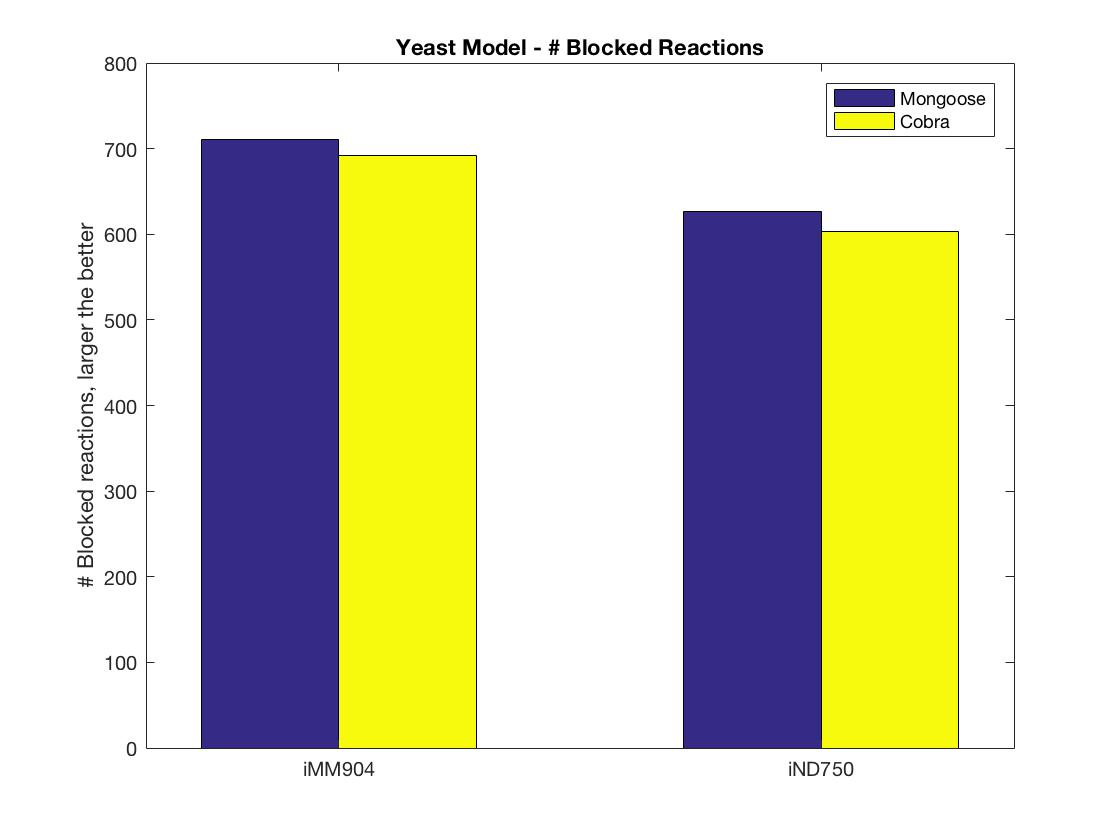
\includegraphics[width=1.0\textwidth]{yeast_no_blocked_reaction.jpg}
%      	\caption{\textit{Number of blocked reactions for yeast models.}}
%	\end{figure}
%	\begin{figure}[H]
%  		\centering
%      	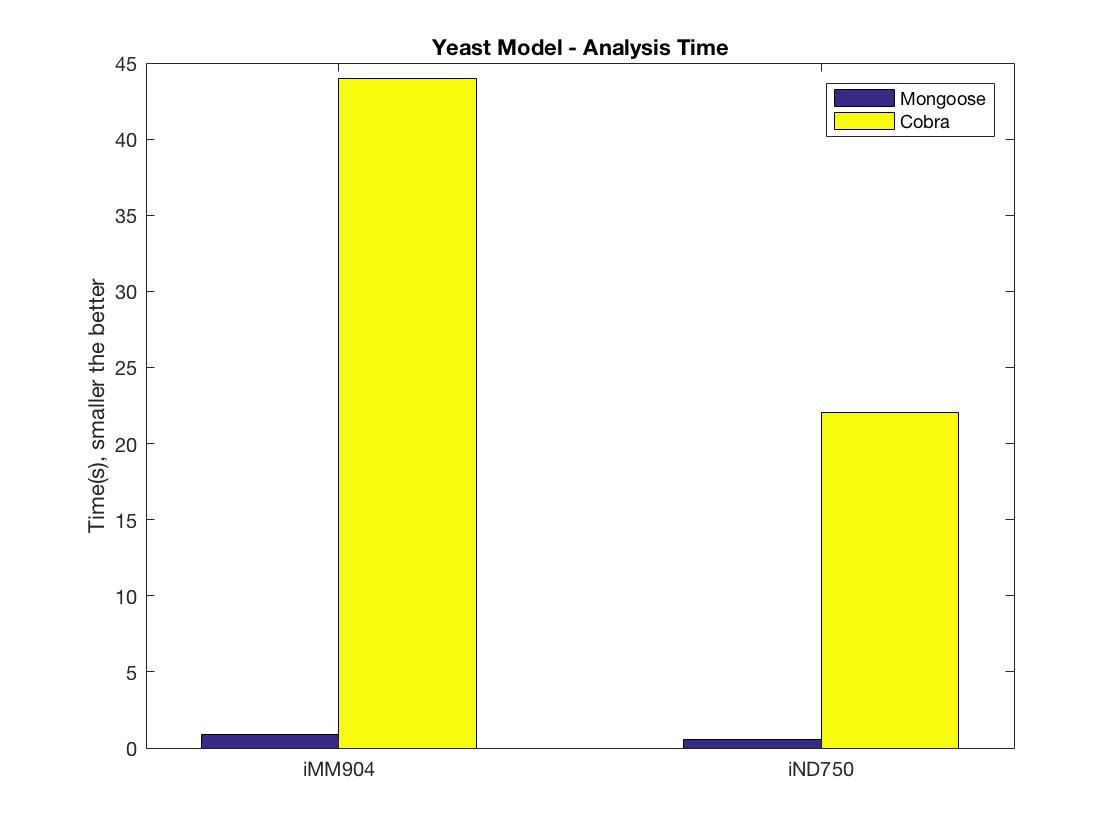
\includegraphics[width=1.0\textwidth]{yeast_time.jpg}
%      	\caption{\textit{Analysis time for yeast models.}}
%	\end{figure}
%	~\\In order to compare two tools in a fair manner, in our first step we use results from two yeast models as reference. From figure 4, we can see that Mongoose slights beats Cobra in finding the number of blocked reactions by 10\% while in terms of analysis time in figure 5, cobra takes much more time.
%	\begin{figure}[H]
%  		\centering
%      	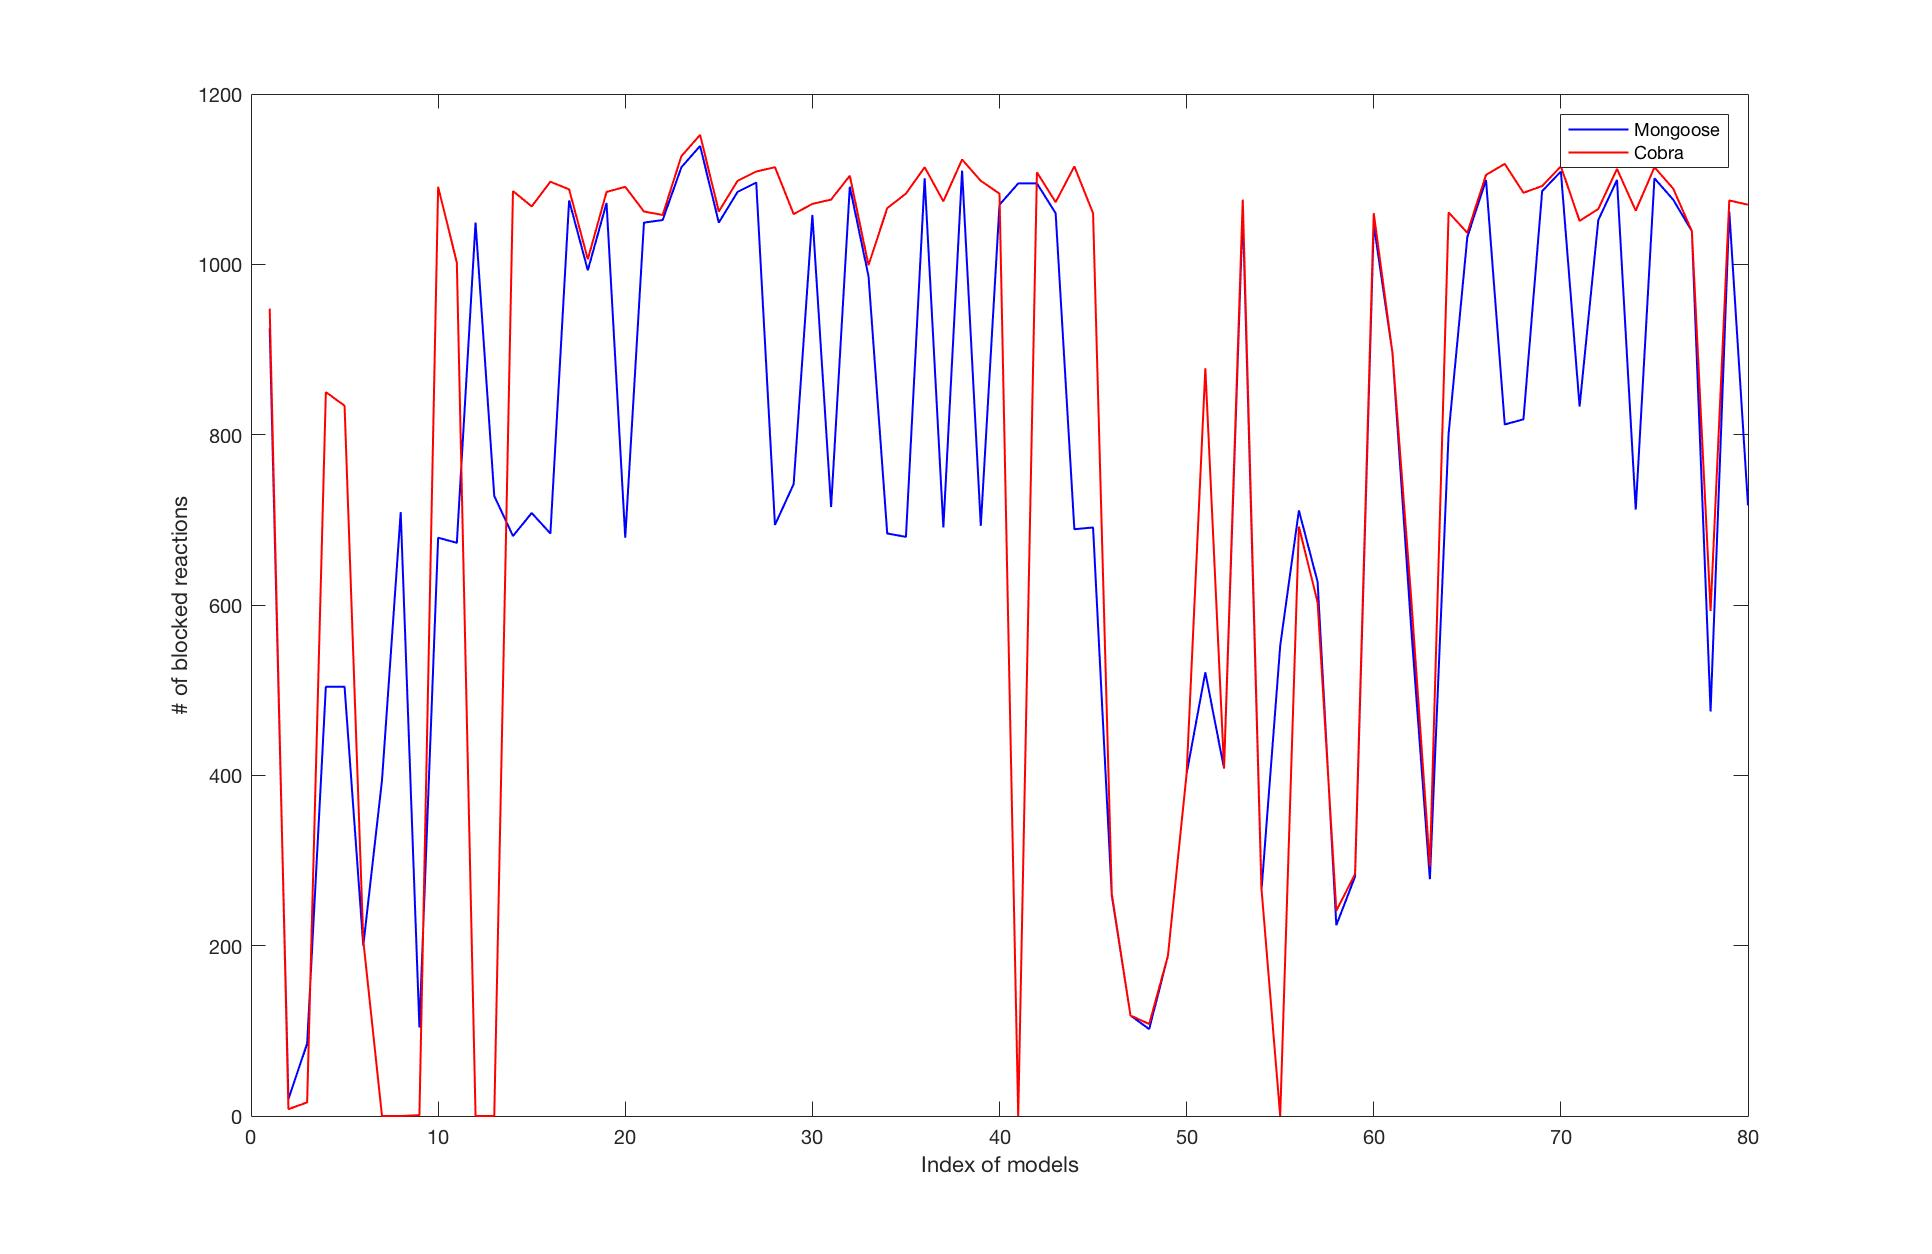
\includegraphics[width=1.0\textwidth]{all_model_rxn.jpg}
%      	\caption{\textit{Number of blocked reactions for all 80 BIGG models.}}
%	\end{figure}
%	\begin{figure}[H]
%  		\centering
%      	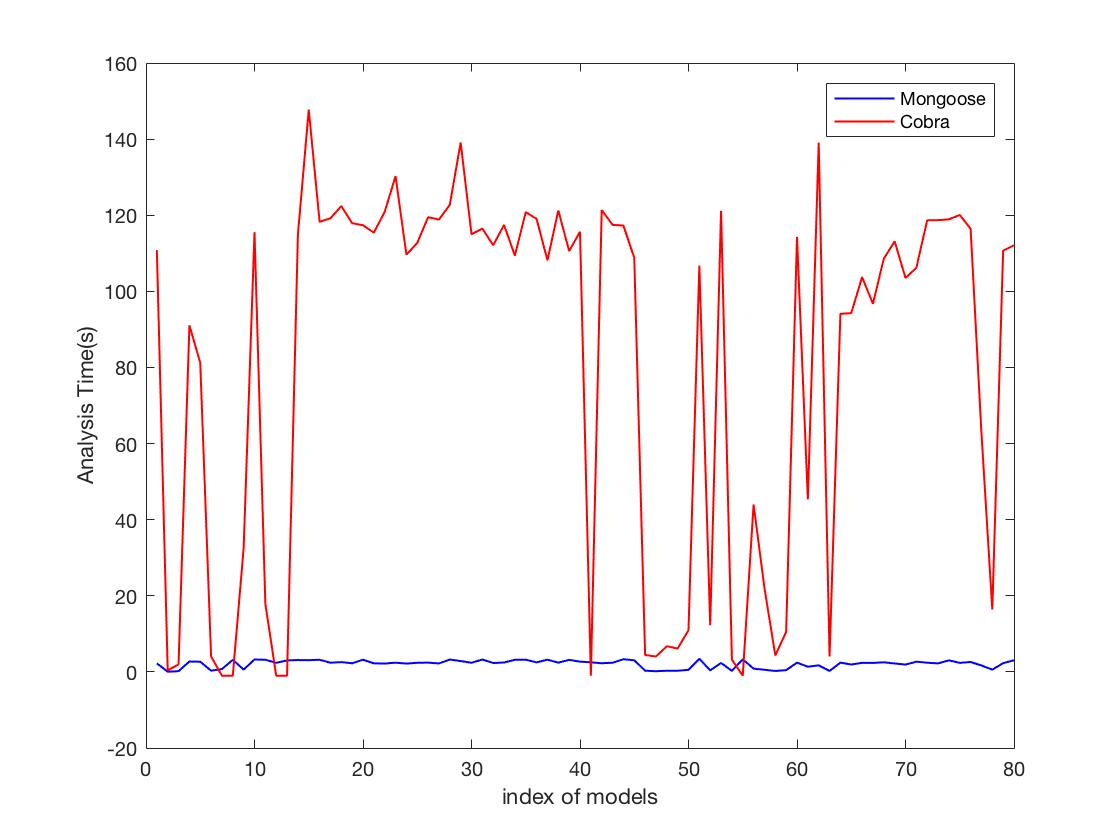
\includegraphics[width=1.0\textwidth]{all_model_ana_time.jpg}
%      	\caption{\textit{Analysis time for all 80 BIGG models.}}
%	\end{figure}
%	~\\Here regarding the result from 2 yeast models, Mongoose takes 1 point over cobra, but another result tells a different answer when we put all models from UCSD repository for analysis. From figure 6, we can see that the average performance regarding to number of blocked reactions found, Cobra actually performs the same or even better than Mongoose on average. This may be because more models are more compatible with Cobra since it has been developed for a long time since 2007 compared with Mongoose as a new challenger in 2014. However, Mongoose reveals the inconsistencies and irreproducibility of Cobra using floating arithmetic, makes sense in most applications, but not metabolic network analysis with the stoichiometric coefficients that are ratios of small integers.\\
%	\begin{figure}[H]
%  		\centering
%      	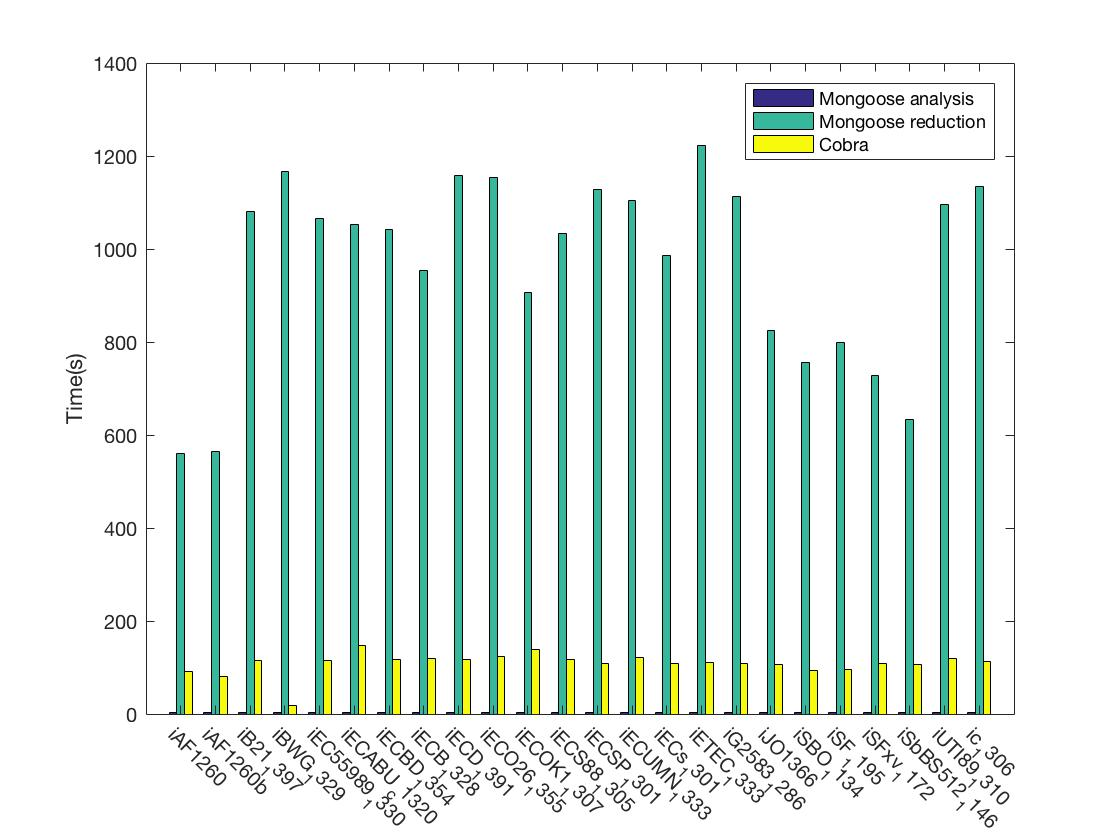
\includegraphics[width=1.0\textwidth]{selected_model_time.jpg}
%      	\caption{\textit{Time cost when network reduction is counted for Mongoose. 24 models with different sizes are taken for example.}}
%	\end{figure}
%	~\\When it comes to the analysis time, figure 7 shows the great advantage Mongoose keeps over Cobra. Though Mongoose takes far less time in analysis, from figure 8, if we count the network reduction time into consideration, Mongoose takes 18 minutes on average for each model and 25 hours for all 80 models, which is very expensive compared with Cobra 1.35 minutes for each model on average and 1.80 hours for all 80 models. This is because Cobra does the whole analysis process for each model every time while Mongoose can save the reduced model for future use, showing great efficiency and sustainability. To sum up, with exact arithmetic computation method and reusable reduced model, Mongoose performs better than Cobra in its consistency and efficiency. But in terms of accuracy, though Mongoose slightly beats Cobra on yeast models, on average gives almost same results as Cobra does. It is hard to tell exactly which one is better.
As last part of the \textbf{easy goal} of our projects we went through lab of module 4 in the \textit{System and Network Biology} workshop. Subsection \textbf{4.1} contains the results of the lab. After that we explain the results of our \textbf{hard goal} in subsection \textbf{4.2}. Finally, for our \textbf{stretch goal} we went to similar process as our hard goal for all the models available from the In Sili-co Organisms repository. Results of the stretch goal is available in subsection \textbf{4.3}.
	\subsection{Cobra}
	In order to learn how constraint-based models of bacterial metabolism are implemented using state of the art modeling tools, we utilizing the Cobra toolbox that was developed by Prof. Bernhard Palsson’s group at the University of California, San Diego in the Nature paper 'Quantitative prediction of cellular metabolism with constraint‐based models: the COBRA Toolbox.'$\cite{Becker20}$

	~\\The goal of the first part of the laboratory is to load the SBML model of E. coli iJR904 and to evaluate its contents using\\$>>model=readCbModel('iJR904')$;\\After loading the model, we can identify (i) the number of genes(904), metabolites(761) and reactions(1075). (ii) the rank(743) of the resulting matrix\\$>>rank(full(model.S))$;\\(iii) degree of freedom(332) (i.e the extent to which the model is underdetermined)[x]\\$degree of freedom = number of reactions - rank of matrix$\\(iv) plot the matrix\\$>>spy(model.S)$.
	\begin{figure}[H]
  		\centering
      	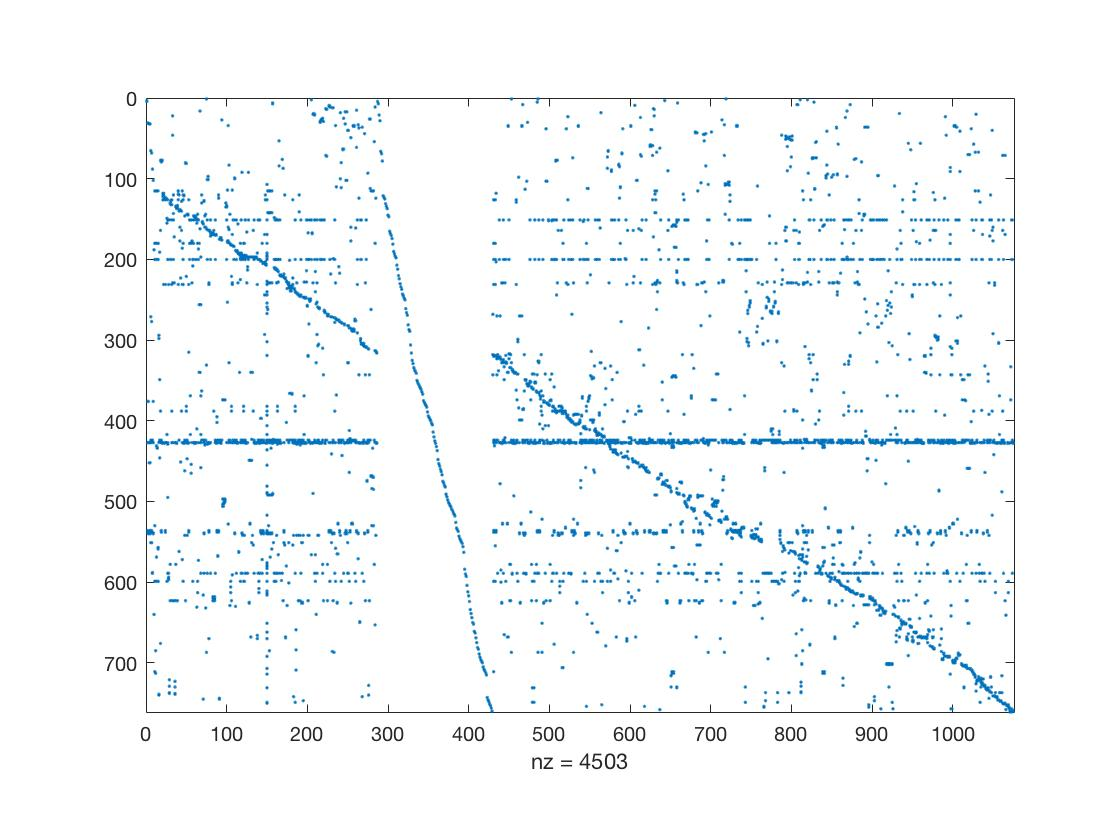
\includegraphics[width=0.8\textwidth]{matrix_plot.jpg}
      	\caption{\textit{Plot of stoichiometry matrix where we can find highly connected metabolites.}}
	\end{figure}
	~\\Then we tried to solve the E. coli model using the FBA approach where the biomass maximization is the objective function.\\$>>solution1 = optimizeCbModel(model)$;\\
	The growth rate is $0.9219 hr^{-1}$\\\\
	Here we compare the biomass yield for different amount of glucose uptake.\\
	$>>model2=changeRxnBounds(model,'EX\_glc\_\_D\_e',[-1],'l');$\\
	Biomass yield is 0.0604389 when glucose uptake is $1 mmol/gdw hr$
	and it increases linearly 0.539113 when glucose uptake is raised to $6 mmol/gdw hr$.\\
	~\\Next we changed objective function for the linear programming problem to that of maximizing the rate of ethanol production to maximize ethanol yield\\
	$>>model3=changeObjective(model,{'BiomassEcoli','EX\_etoh(e)'},[0,1]);$\\
	we find the reaction is be under eraobic condition in this case and the growth rate is be 0.\\
	~\\If we force the environment to be in anaerobic condition (i.e. set the oxygen taken to be 0)\\$>>model4=changeRxnBounds(model,'EX\_o2\_e',[0],'l');$\\We find that the ethanol yield is actually smaller than the result above, which means the maximum of ethanol yield may not be necessarily under anaerobic condition.\\
	\begin{figure}[H]
  		\centering
      	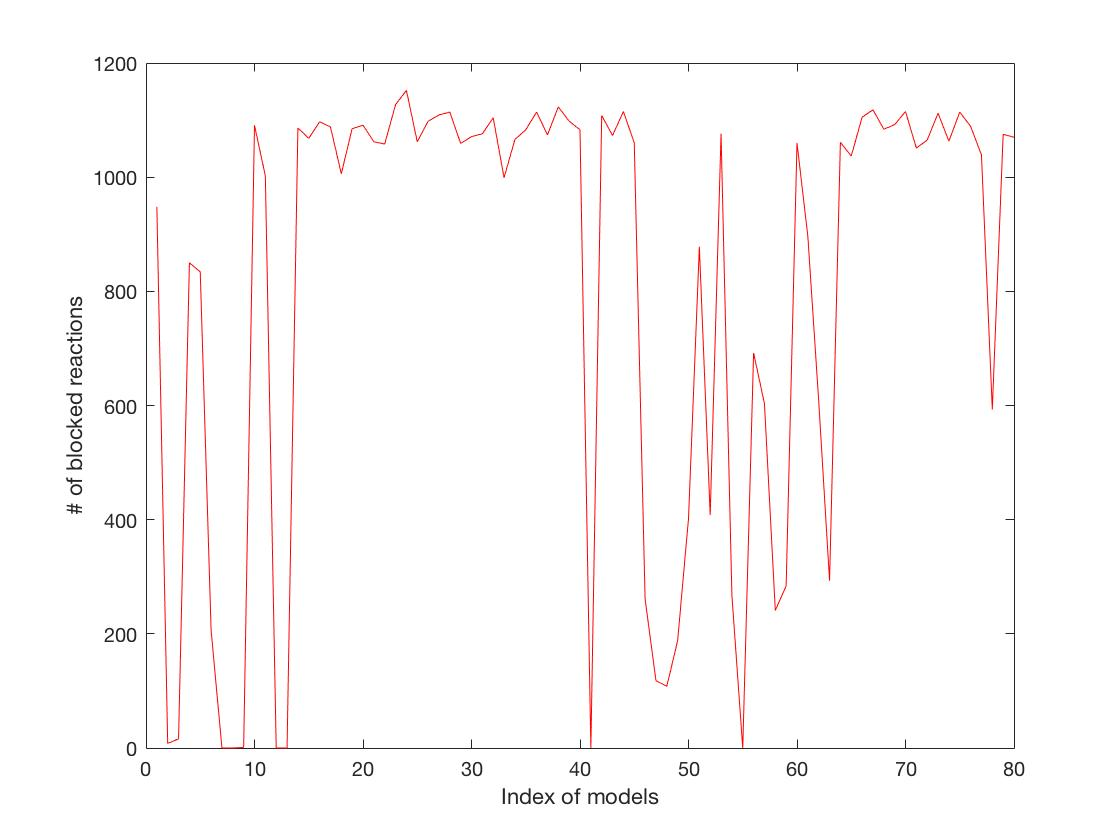
\includegraphics[width=0.8\textwidth]{cobra_all_model_reaction.jpg}
      	\caption{\textit{Number of reactions for all models found by cobra.}}
	\end{figure}
%	\begin{figure}[H]
%  		\centering
%      	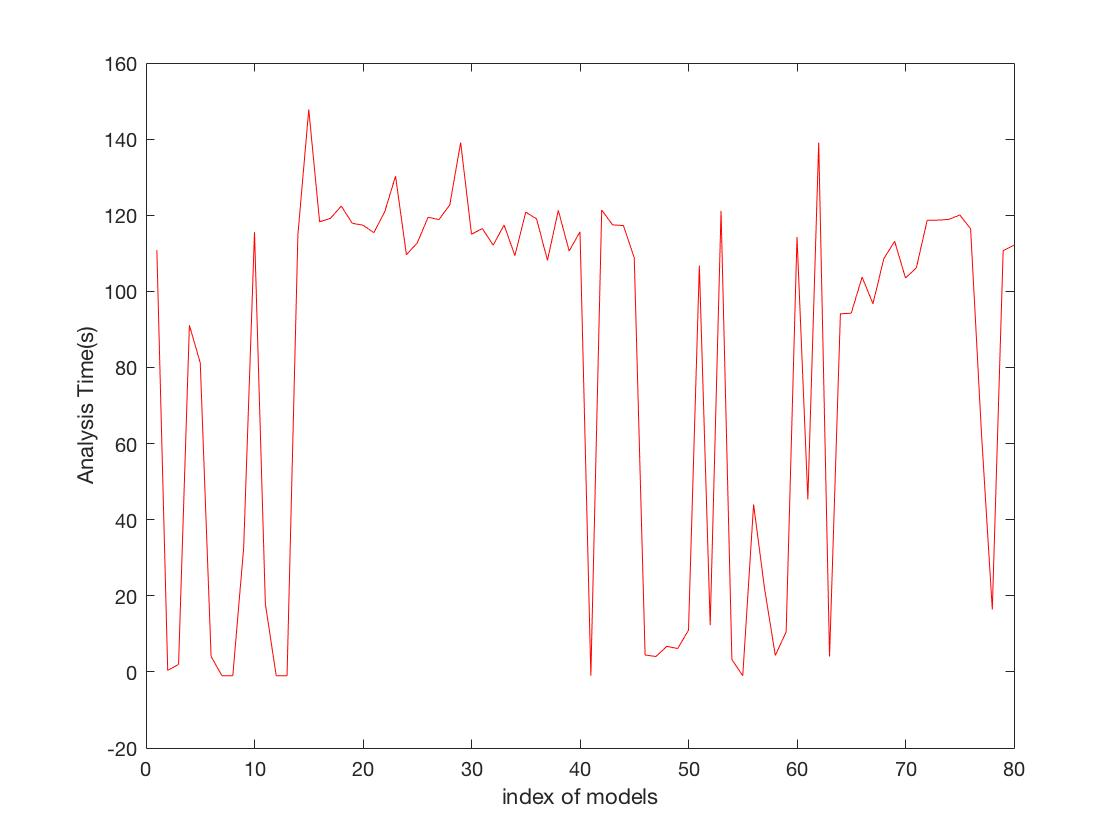
\includegraphics[width=0.8\textwidth]{cobra_all_model_time.jpg}
%      	\caption{\textit{Analysis time for all models by cobra.}}
%	\end{figure}
	~\\After having a basic understading of FBA and cobra functions, we focused on the number of blocked reactions using yeast models iMM904, IND750 as gold standard data and all models from http://bigg.ucsd.edu/models. One interesting thing we find is that for some models, cobra cannot give the correct result in a reasonable time (e.g. 2 hours).
	\begin{center}
	\begin{tabular}{|c|c|c|} 
	 \hline
	 Yeast Model & \# Blocked Reactions & Analysis Time(s)\\
	 \hline 
	 iMM904 & 692 & 43.9767 \\
	 IND750 & 603 & 22.0524 \\
	 \hline
	\end{tabular}
	\end{center}
	\subsection{Mongoose}
	~\\ As part of our hard goal after installation of MONGOOSE, we analyzed the structure of the model \textit{iJR904} of \textit{E. coli}. For next part we needed a gold standard data in order to compare results of COBRA adn MONGOOSE. For this purpose we used \textit{yeast} models \textit{iMM904} and \textit{IND750} as our gold standard models. Finally, we repeat the same process for all  models available from the In Sili-co Organisms repository.In the following sections we used number of blocked reactions, obtained by COBRA and MONGOOSE, for the  comparison.

	~\\For model \textit{iJR904} of \textit{E. coli} after parsing the model and reducing the network we obtained following results. This model contains 761 metabolites and 1075 reactions. Also, MONGOOSE found 7 stociometrically-blocked reactions, 247 topologically-blocked reaction and 56 irreversibility-blocked reactions in this model. Totally 310 blocked reactions. In addition MONGOOSE found 17 semi-blocked reaction (Commands have been used for these results is available in appendix).

	~\\By repeating the same procedure on \textit{yeast} models \textit{iMM904} and \textit{iND750} we found out \textit{iMM904} contains 711 blocked reactions and \textit{ iND750} contains 627 blocked reactions compare to COBRA's result for these models which respectively was 692 and 603 blocked reactions. 
	\begin{center}

	%\caption{MONGOOSE results for \textit{iMM904} and \textit{iND750}}
	\label{yestResults}
	    \begin{tabular}{|c|c|c|}
	        \hline
	        Model                         & iMM904 & iND770 \\ \hline
	        Metabolites                & 1226  & 1059   \\ 
	        Reactions                  & 1577   & 1266   \\ 
	        Stoichiometrically Blocked & 108    & 104    \\ 
	        Topologically Blocked      & 382    & 335    \\ 
	        Irreversibility Blocked    & 221    & 188    \\ 
	        Total Blocked Reactions    & 711    & 627    \\ 
	        Semi-Blocked Reactions     & 25     & 18     \\
	        \hline
	    \end{tabular}
	\end{center}

	~\\Finally we repeat last steps on all models available on the In Sili-co Organisms repository. The following table includes results couple of these models. Results of all models are available in table $\ref{allModels}$ in appendix.

	\begin{table}[htb]
	\centering
	\caption{Number of blockages in the first ten models which are availbe on the In Sili-co Organisms repository}
	\label{my-label}
	\resizebox{18cm}{!}{
	\begin{tabular}{|l|l|l|l|l|l|l|l|l|l|l|}
	\hline
	Model              & RECON1 & STM\_v1\_0 & e\_coli\_core & iAB\_RBC\_283 & iAF1260 & iAF1260b & iAF692 & iAF987 & iAPECO1\_1312 & iAT\_PLT\_636 \\ \hline
	Stoichiometrically & 195    & 12         & 0             & 2             & 13      & 13       & 1      & 9      & 15            & 0             \\ \hline
	Topologically      & 872    & 482        & 20            & 83            & 405     & 405      & 182    & 291    & 624           & 104           \\ \hline
	Irreversibility    & 579    & 80         & 0             & 0             & 86      & 86       & 17     & 94     & 70            & 0             \\ \hline
	SemiBlocked        & 44     & 42         & 2             & 9             & 32      & 29       & 21     & 32     & 46            & 8             \\ \hline
	Combined           & 1646   & 574        & 20            & 85            & 504     & 504      & 200    & 394    & 709           & 104           \\ \hline
	\end{tabular}
	}
	\end{table}
	\subsection{Compairson and Analysis}
	~\\We performed experiments on two popular toolboxes for metabolic network analysis and explored why differences arise between results shown above. According to MONGOOSE paper $\cite{Leonid19}$, we know that the biggest difference between them is that Cobra uses floating arithmetic while Mongoose uses exact arithmetic (or rational arithmetic) for computation.  But we have to note that the stoichiometric matrix in the constraint-based model contains rational numbers$\cite{Leonid19}$. Also, (we think) it is reasonable to assume that vector of fluxes should contains rational numbers as well. Hence, we can assume that, using rational arithmetic for these models will preserve the accuracy in our results. In the following section we compared the number of blocked reactions which was obtained by MONGOOSE and COBRA. 
		~\\In order to compare two tools in a fair manner, in our first step we use results from two yeast models as reference. From figure 4, we can see that Mongoose slights beats Cobra in finding the number of blocked reactions by 10\% while in terms of analysis time in figure 5, cobra takes much more time.
	\begin{figure}[H]
  		\centering
      	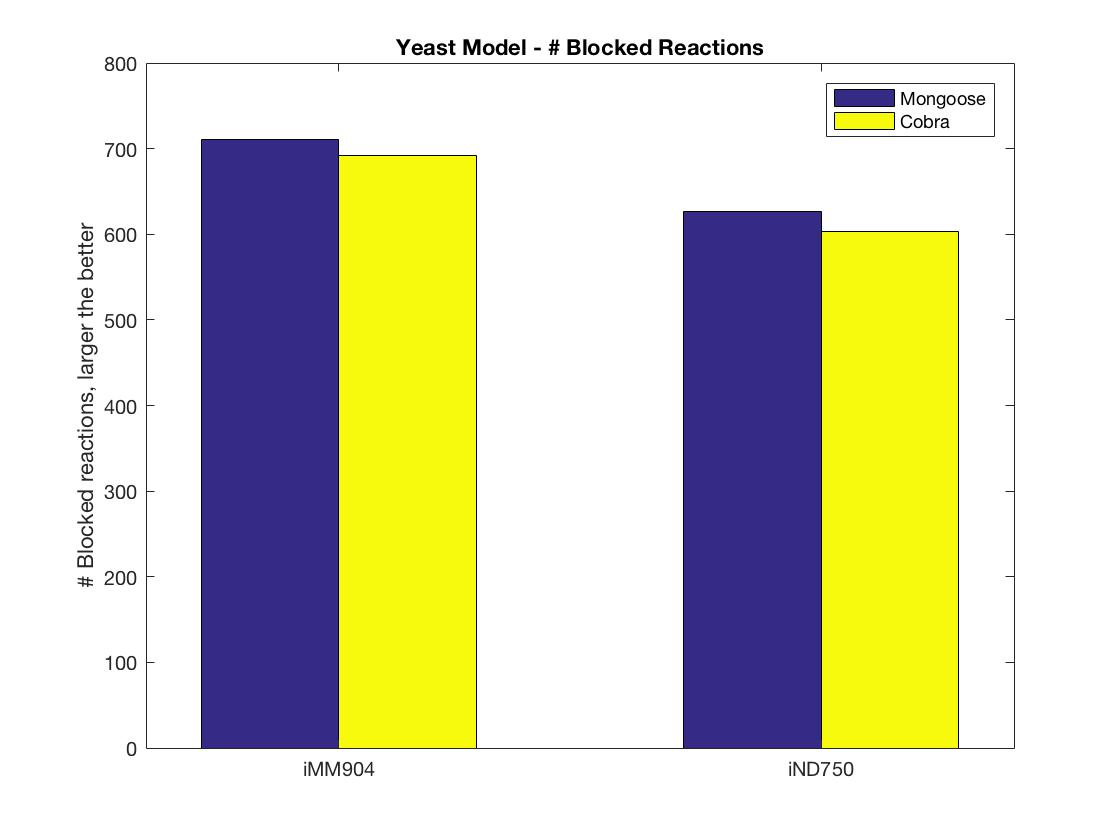
\includegraphics[width=1\textwidth]{yeast_no_blocked_reaction.jpg}
      	\caption{\textit{Number of blocked reactions for yeast models.}}
	\end{figure}
	\begin{figure}[H]
  		\centering
      	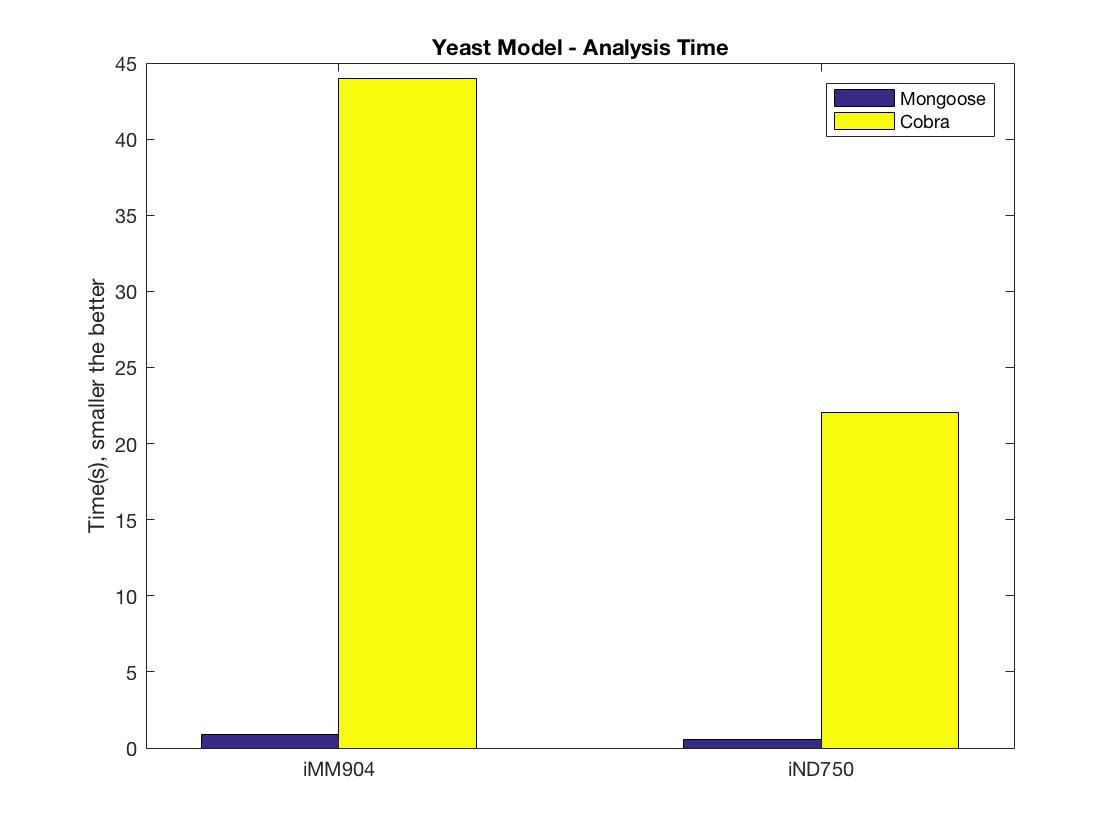
\includegraphics[width=1\textwidth]{yeast_time.jpg}
      	\caption{\textit{Analysis time for yeast models.}}
	\end{figure}
	~\\Here regarding the result from 2 yeast models, Mongoose takes 1 point over cobra, but another result tells a different answer when we put all models from UCSD repository for analysis. From figure 6, we can see that the average performance regarding to number of blocked reactions found, Cobra actually performs the same or even higher than Mongoose on average.
	% This may be because more models are more compatible with Cobra since it has been developed for a long time since 2007 compared with Mongoose as a new challenger in 2014. 
However, Mongoose reveals the inconsistencies and irreproducibility of Cobra using floating arithmetic, makes sense in most applications, but not metabolic network analysis with the stoichiometric coefficients that are ratios of small integers.\\
	\begin{figure}[H]
  		\centering
      	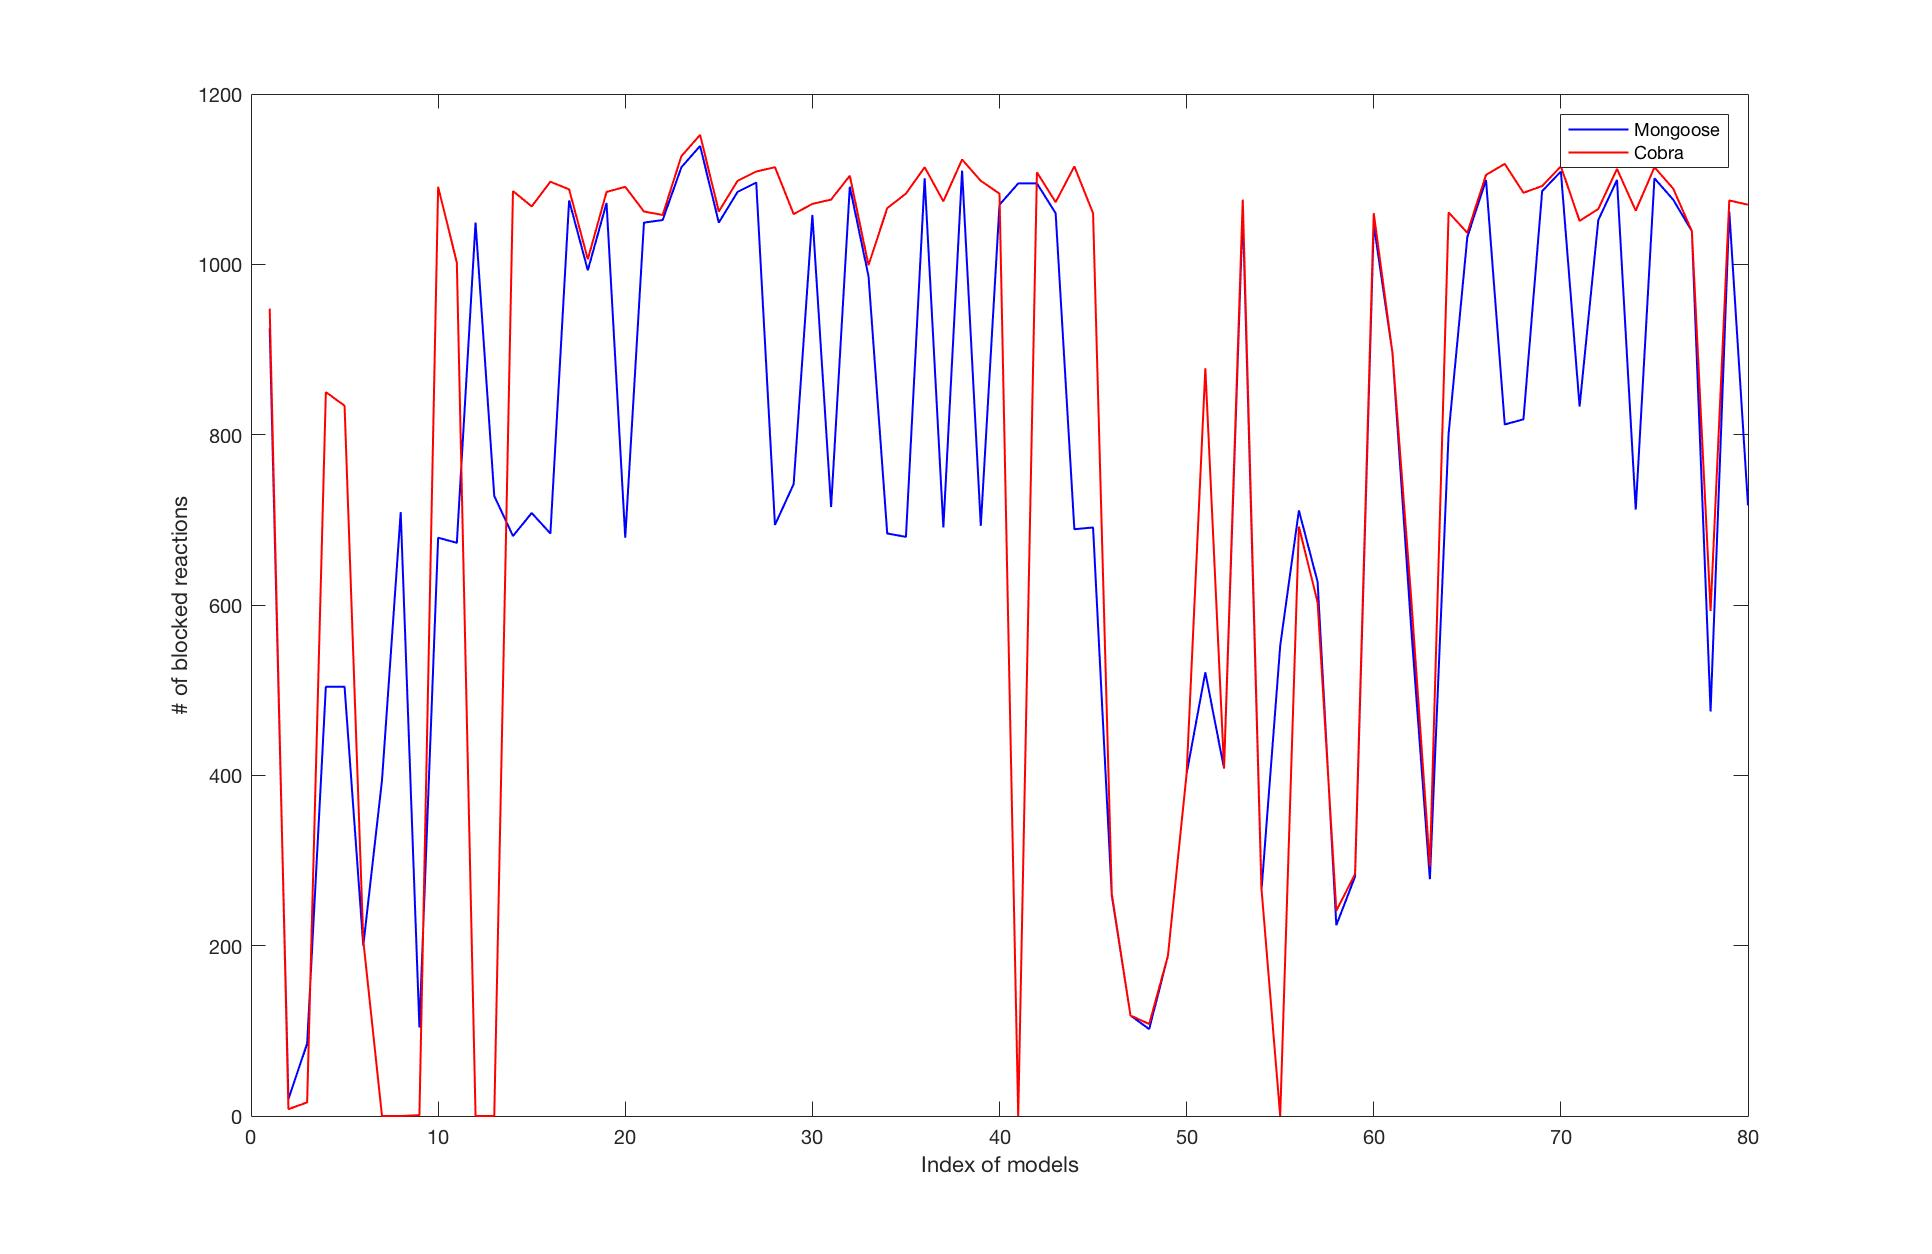
\includegraphics[width=0.8\textwidth]{all_model_rxn.jpg}
      	\caption{\textit{Number of blocked reactions for all 80 BIGG models.}}
	\end{figure}
	\begin{figure}[H]
  		\centering
      	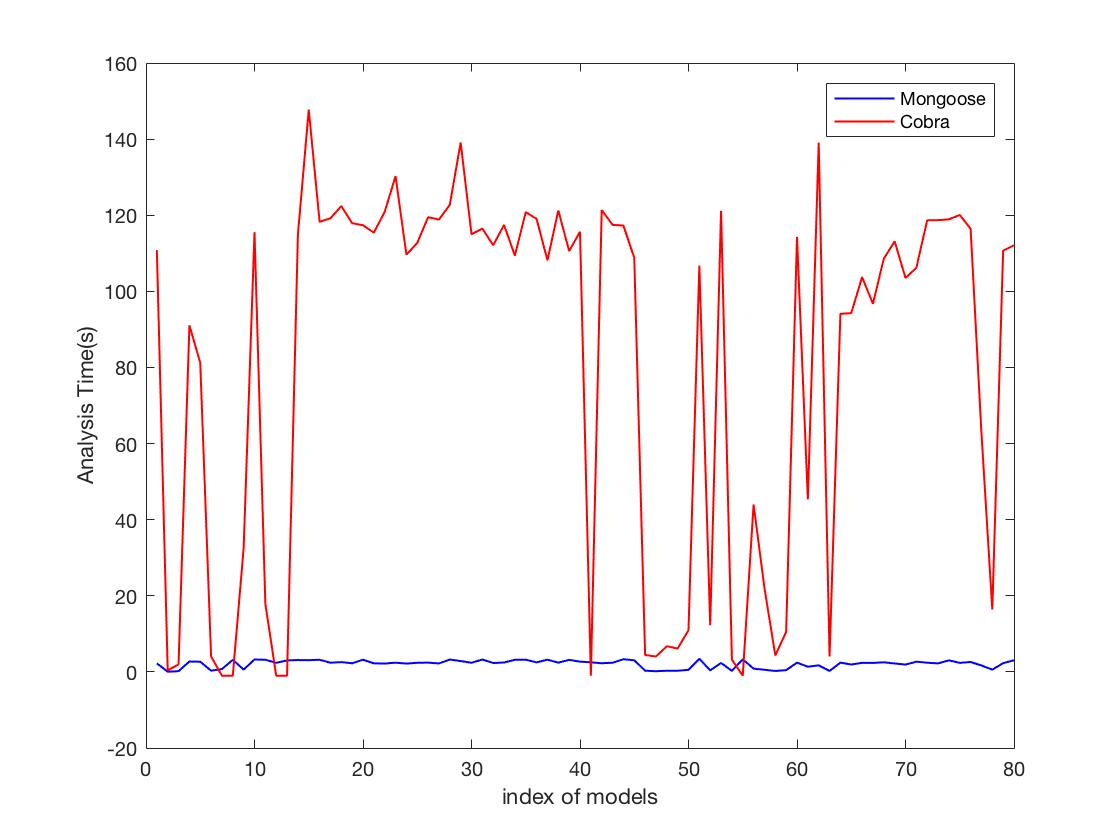
\includegraphics[width=0.8\textwidth]{all_model_ana_time.jpg}
      	\caption{\textit{Analysis time for all 80 BIGG models.}}
	\end{figure}
	\begin{figure}[H]
  		\centering
      	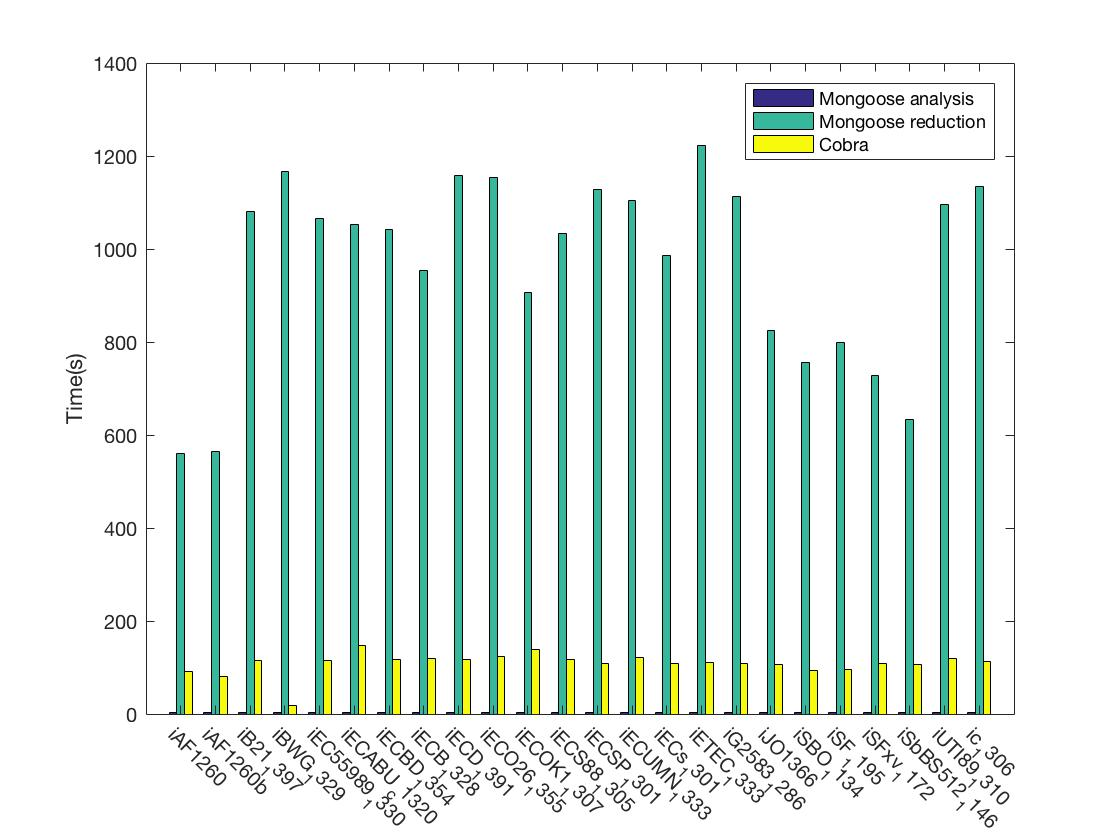
\includegraphics[width=1.0\textwidth]{selected_model_time.jpg}
      	\caption{\textit{Time cost when network reduction is counted for Mongoose. 24 models with different sizes are taken for example.}}
	\end{figure}
	~\\When it comes to the analysis time, figure 7 shows the great advantage Mongoose keeps over Cobra. Though Mongoose takes far less time in analysis, from figure 8, if we count the network reduction time into consideration, Mongoose takes 18 minutes on average for each model and 25 hours for all 80 models, which is very expensive compared with Cobra 1.35 minutes for each model on average and 1.80 hours for all 80 models. This is because Cobra does the whole analysis process for each model every time while Mongoose can save the reduced model for future use, showing great efficiency and sustainability. To sum up, with exact arithmetic computation method and reusable reduced model, Mongoose performs better than Cobra in its consistency and efficiency. But in terms of accuracy, though Mongoose slightly beats Cobra on yeast models, on average gives almost same results as Cobra does. It is hard to tell exactly which one is better.
	%==========Conclusion==========%
	\newpage
	\section{Conclusion}
	~\\In this project we obtained a basic knowledge about metabolic networks, constraint-based models and flux balance analysis$\cite{Chalancon1}$ $\cite{Conde3}$ $\cite{Klamt10}$ $\cite{Orth12}$ $\cite{Hinton18}$. Also, we learned about two analysis toolboxes COBRA $\cite{Becker20}$ and MONGOOSE $\cite{Leonid19}$, and compared them from our point of view.\\
	In general, we found our, it is hard to compare MONGOOSE and COBRA, since both toolboxes have their own advantage and disadvantages. COBRA has variety of functions compare to MONGOOSE. However, MONGOOSE ravels novel structure features of constraint-based models. MONGOOSE is able to identify blockages based on their cause and even fix those blockages. It is also able to identify reversible reaction which only can satisfy the model's constraints in one direction. Moreover, compare to COBRA which using float-base arithmetic, MONGOOSE uses exact arithmetic which cause consistency in analysis. In addition, even though COBRA usually take less time to perform due to usage of floating-point arithmetic, MONGOOSE detect a lot of structure features, in one step , when we are reducing the network and after that we have better performance (time-wise) than COBRA. Also, we have to mention that COBRA can be easier to install and use than MONGOOSE for researchers with less knowledge of computer since it uses MATLAB. Overall, based on our observation in this project, the critical structural features of model which are revealed by MONGOOSE can give us better understanding of the model and it would cause more accurate analysis. 
	%==========References==========%
	\newpage
	\addcontentsline{toc}{section}{References}
	\renewcommand\refname{References}
	\raggedright
	\bibliographystyle{unsrt}
	\bibliography{report}
	%==========Appendix==========%
	\newpage
	\section{Appendix}
	The following table containts MOONGOOSE analysis that we had for all models available from the In Sili-co Organisms repository.
		\begin{table}[!htbp]
\caption{This table contains results of all models}
\label{allModels}
\resizebox{\textwidth}{!}{

\begin{tabular}{|l|l|l|l|l|l|l|l|}
\hline
	Model & Reactions & Metabolites & Stochio. Blocked & Topo. Blocked & Irrev. Blocked & SemiBlocked & Combined (Blocked) \\
	\hline
	RECON1 & 2766 & 3741 & 195 & 872 & 579 & 44 & 1646 \\
	STM\_v1\_0 & 1802 & 2545 & 12 & 482 & 80 & 42 & 574 \\
	e\_coli\_core & 72 & 95 & 0 & 20 & 0 & 2 & 20 \\
	iAB\_RBC\_283 & 342 & 469 & 2 & 83 & 0 & 9 & 85 \\
	iAF1260 & 1668 & 2382 & 13 & 405 & 86 & 32 & 504 \\
	iAF1260b & 1668 & 2388 & 13 & 405 & 86 & 29 & 504 \\
	iAF692 & 628 & 690 & 1 & 182 & 17 & 21 & 200 \\
	iAF987 & 1109 & 1285 & 9 & 291 & 94 & 32 & 394 \\
	iAPECO1\_1312 & 1942 & 2735 & 15 & 624 & 70 & 46 & 709 \\
	iAT\_PLT\_636 & 738 & 1008 & 0 & 104 & 0 & 8 & 104 \\
	iB21\_1397 & 1943 & 2741 & 14 & 590 & 75 & 45 & 679 \\
	iBWG\_1329 & 1949 & 2741 & 18 & 581 & 74 & 47 & 673 \\
	iCHOv1 & 4456 & 6663 & 53 & 1872 & 193 & 57 & 2118 \\
	iE2348C\_1286 & 1919 & 2703 & 17 & 611 & 80 & 46 & 708 \\
	iEC042\_1314 & 1926 & 2714 & 22 & 605 & 101 & 35 & 728 \\
	iEC55989\_1330 & 1953 & 2756 & 14 & 597 & 70 & 47 & 681 \\
	iECABU\_c1320 & 1942 & 2731 & 15 & 623 & 70 & 46 & 708 \\
	iECBD\_1354 & 1952 & 2748 & 14 & 595 & 75 & 45 & 684 \\
	iECB\_1328 & 1951 & 2748 & 12 & 594 & 68 & 46 & 674 \\
	iECDH10B\_1368 & 1947 & 2742 & 24 & 576 & 80 & 48 & 680 \\
	iECDH1ME8569\_1439 & 1950 & 2755 & 15 & 582 & 90 & 46 & 687 \\
	iECD\_1391 & 1943 & 2741 & 14 & 590 & 75 & 45 & 679 \\
	iECED1\_1282 & 1929 & 2706 & 16 & 617 & 82 & 45 & 715 \\
	iECH74115\_1262 & 1918 & 2694 & 16 & 615 & 69 & 44 & 700 \\
	iECIAI1\_1343 & 1968 & 2765 & 18 & 598 & 72 & 47 & 688 \\
	iECIAI39\_1322 & 1953 & 2721 & 16 & 649 & 104 & 46 & 769 \\
	iECNA114\_1301 & 1927 & 2718 & 19 & 596 & 70 & 45 & 685 \\
	iECO103\_1326 & 1958 & 2758 & 18 & 599 & 77 & 46 & 694 \\
	iECO111\_1330 & 1959 & 2760 & 20 & 601 & 87 & 47 & 708 \\
	iECO26\_1355 & 1965 & 2780 & 17 & 596 & 81 & 47 & 694 \\
	iECOK1\_1307 & 1941 & 2729 & 15 & 634 & 93 & 37 & 742 \\
	iECP\_1309 & 1941 & 2739 & 13 & 621 & 73 & 45 & 707 \\
	iECS88\_1305 & 1942 & 2729 & 19 & 626 & 70 & 46 & 715 \\
	iECSE\_1348 & 1957 & 2768 & 17 & 589 & 69 & 47 & 675 \\
	iECSF\_1327 & 1951 & 2742 & 14 & 583 & 61 & 47 & 658 \\
	iECSP\_1301 & 1920 & 2712 & 17 & 596 & 71 & 44 & 684 \\
	iECUMN\_1333 & 1935 & 2740 & 13 & 598 & 69 & 45 & 680 \\
	iECW\_1372 & 1973 & 2782 & 14 & 602 & 70 & 47 & 686 \\
	iECs\_1301 & 1923 & 2720 & 17 & 593 & 81 & 45 & 691 \\
	iEKO11\_1354 & 1972 & 2778 & 14 & 597 & 77 & 47 & 688 \\
	iETEC\_1333 & 1962 & 2756 & 17 & 605 & 71 & 46 & 693 \\
	iEcDH1\_1363 & 1949 & 2750 & 14 & 583 & 87 & 46 & 684 \\
	iEcE24377\_1341 & 1972 & 2763 & 17 & 619 & 69 & 47 & 705 \\
		iEcHS\_1320 & 1963 & 2753 & 14 & 600 & 68 & 46 & 682 \\
	iEcSMS35\_1347 & 1947 & 2746 & 14 & 611 & 68 & 46 & 693 \\
	iEcolC\_1368 & 1969 & 2768 & 18 & 601 & 70 & 46 & 689 \\
	iG2583\_1286 & 1919 & 2704 & 16 & 604 & 71 & 46 & 691 \\
	iHN637 & 698 & 785 & 3 & 253 & 18 & 11 & 274 \\
	iIT341 & 485 & 554 & 1 & 113 & 4 & 15 & 118 \\
	iJB785 & 768 & 849 & 2 & 107 & 10 & 25 & 119 \\
	iJN678 & 795 & 863 & 5 & 148 & 17 & 13 & 170 \\
	iJN746 & 907 & 1054 & 3 & 220 & 15 & 13 & 238 \\
	iJO1366 & 1805 & 2583 & 13 & 443 & 65 & 45 & 521 \\
	iJR904 & 761 & 1075 & 7 & 247 & 56 & 17 & 310 \\
	iLB1027\_lipid & 2172 & 4456 & 39 & 170 & 190 & 33 & 399 \\
	iLF82\_1304 & 1938 & 2726 & 13 & 627 & 82 & 46 & 722 \\
	iLJ478 & 570 & 652 & 3 & 181 & 4 & 13 & 188 \\
	iML1515 & 1877 & 2712 & 14 & 479 & 59 & 42 & 552 \\
	iMM1415 & 2775 & 3726 & 38 & 925 & 215 & 52 & 1178 \\
	iMM904 & 1226 & 1577 & 108 & 382 & 221 & 25 & 711 \\
	iND750 & 1059 & 1266 & 104 & 335 & 188 & 18 & 627 \\
	iNF517 & 650 & 754 & 0 & 207 & 17 & 13 & 224 \\
	
\hline
\end{tabular}}
\end{table}
\begin{table}[!htbp]
\resizebox{\textwidth}{!}{
\begin{tabular}{|l|l|l|l|l|l|l|l|}
\hline
	Model & Reactions & Metabolites & Stochio. Blocked & Topo. Blocked & Irrev. Blocked & SemiBlocked & Combined (Blocked) \\
	\hline
	iNJ661 & 825 & 1025 & 3 & 207 & 85 & 21 & 295 \\
	iNRG857\_1313 & 1943 & 2735 & 15 & 624 & 70 & 46 & 709 \\
	iPC815 & 1552 & 1961 & 28 & 587 & 121 & 32 & 736 \\
	iRC1080 & 1706 & 2191 & 37 & 402 & 133 & 34 & 572 \\
	iSB619 & 655 & 743 & 2 & 209 & 17 & 17 & 228 \\
	iSBO\_1134 & 1908 & 2591 & 25 & 667 & 109 & 26 & 801 \\
	iSDY\_1059 & 1888 & 2539 & 31 & 676 & 139 & 23 & 846 \\
	iSFV\_1184 & 1917 & 2621 & 22 & 690 & 121 & 36 & 833 \\
	iSF\_1195 & 1917 & 2630 & 23 & 670 & 119 & 31 & 812 \\
	iSFxv\_1172 & 1918 & 2638 & 28 & 671 & 119 & 35 & 818 \\
			iSFxv\_1172 & 1918 & 2638 & 28 & 671 & 119 & 35 & 818 \\
	iSSON\_1240 & 1936 & 2693 & 20 & 631 & 100 & 40 & 751 \\
	iS\_1188 & 1914 & 2619 & 23 & 679 & 125 & 34 & 827 \\
	iSbBS512\_1146 & 1910 & 2591 & 18 & 702 & 113 & 34 & 833 \\
	iUMN146\_1321 & 1942 & 2735 & 15 & 627 & 70 & 46 & 712 \\
	iUMNK88\_1353 & 1969 & 2777 & 16 & 601 & 81 & 47 & 698 \\
	iUTI89\_1310 & 1940 & 2725 & 14 & 627 & 71 & 46 & 712 \\
	iWFL\_1372 & 1973 & 2782 & 14 & 602 & 70 & 47 & 686 \\
	iY75\_1357 & 1953 & 2759 & 15 & 584 & 90 & 46 & 689 \\
	iYL1228 & 1658 & 2262 & 29 & 476 & 200 & 30 & 705 \\
	iYO844 & 990 & 1250 & 3 & 441 & 31 & 17 & 475 \\
	iZ\_1308 & 1923 & 2721 & 17 & 593 & 81 & 45 & 691 \\
	ic\_1306 & 1936 & 2726 & 15 & 628 & 74 & 46 & 717 \\
\hline
\end{tabular}}
\end{table}
\end{document}